\documentclass{article}
\usepackage[utf8]{inputenc}

\title{yo}
\author{shalabh147 }
\date{October 2019}
\usepackage{tikz}
\usetikzlibrary{positioning,arrows}
\usetikzlibrary{shapes.geometric}
\begin{document}



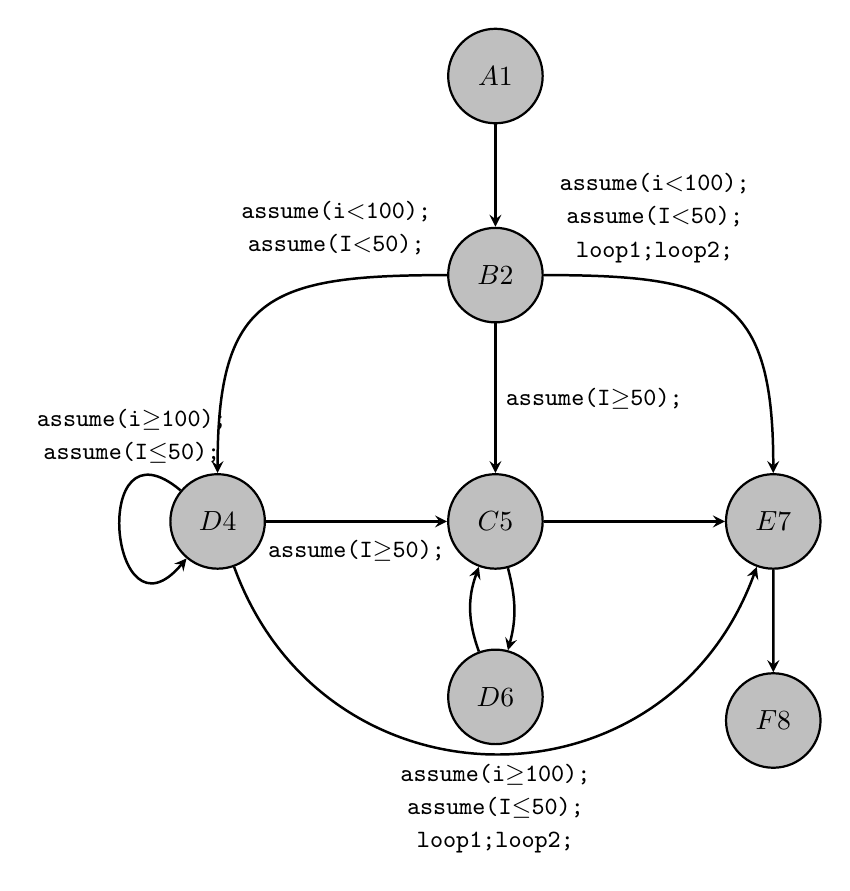
\begin{tikzpicture}[
roundnode/.style={circle, draw=black!100, fill=gray!50,thick, minimum size=12mm},
squarednode/.style={rectangle, draw=black!100, fill=gray!50,thick, minimum size=5mm},
scale=1.4
]
%Nodes
\node[roundnode]      (maintopic)                              {$C5$};
\node[roundnode]        (uppercircle)       [above=1.9cm of maintopic] {$B2$};
\node[roundnode]      (rightsquare)     [right= 2.3cm of maintopic] {$E7$}; 
\node[roundnode]        (lowercircle)       [below=1cm of maintopic] {$D6$};
\node[roundnode]        (uppercircle2)       [above=1.3cm of uppercircle] {$A1$};
\node[roundnode]       (leftcircle)          [left=2.3cm of maintopic] {$D4$};
\node[roundnode]        (newcircle)          [below=1.3cm of rightsquare] {$F8$}; 
%Lines
\draw[->] (uppercircle) edge[->,>=stealth,out=270,in=90,line width=.9pt] node[right] {\small \texttt{assume(I$\geq$50);}} (maintopic);
\draw[->] (uppercircle2) edge[->,>=stealth,out=270,in=90,line width=.9pt] (uppercircle);
\draw[->] (leftcircle) edge[->,>=stealth,out=0,in=180,line width=.9pt] node[below=0.1cm] {\small \texttt{assume(I$\geq$50);}}   (maintopic);
\draw[->] (maintopic) edge[->,>=stealth,out=0,in=180,line width=.9pt] (rightsquare);
\draw[->] (rightsquare) edge[->,>=stealth,out=270,in=90,line width=.9pt] (newcircle);
\draw[->] (uppercircle) edge[->,>=stealth,out=180,in=90,looseness=1.50,line width=.9pt]
node[above=0.2cm,near start,align=center] {\small \texttt{assume(i$<$100);}\\ \small \texttt{assume(I$<$50);}} (leftcircle) ;
\draw[->] (uppercircle) edge[->,>=stealth,out=0,in=90,looseness=1.50,line width=.9pt] node[above=0.1cm,near start,align=center]  {\small \texttt{assume(i$<$100);}\\ \small \texttt{assume(I$<$50);}\\ \small \texttt{loop1;loop2;}}  (rightsquare);
\draw (lowercircle) edge[->,>=stealth,out=110,in=250,line width=.9pt] (maintopic);
\draw[->] (maintopic) edge[->,>=stealth,out=285,in=75,line width=.9pt] (lowercircle);
\draw[->] (leftcircle) edge[->,>=stealth,out=290,in=250,looseness=1.3,line width=.9pt] node[below,align=center] {\small \texttt{assume(i$\geq$100);}\\ \small \texttt{assume(I$\leq$50);}\\
\small \texttt{loop1;loop2;}} (rightsquare);
\draw (leftcircle) edge[->,>=stealth,out=140,in=230,looseness=4.5,line width=.9pt] node[above=0.1cm,near start,align=center] {\small \texttt{assume(i$\geq$100);}\\ \small \texttt{assume(I$\leq$50);}} (leftcircle);
\end{tikzpicture}





\end{document}
